\documentclass[12pt, a4paper]{article}

% ── Packages ──────────────────────────────────────────────────────────────────
\usepackage[margin=2.5cm]{geometry}
\usepackage{graphicx}
\usepackage{amsmath, amssymb}
\usepackage{booktabs}
\usepackage{listings}
\usepackage{xcolor}
\usepackage{hyperref}
\usepackage{enumitem}
\usepackage{tikz}
\usetikzlibrary{arrows.meta, positioning, calc}
\usepackage{float}
\usepackage{caption}

% ── Code listing style ───────────────────────────────────────────────────────
\definecolor{codebg}{RGB}{245,245,245}
\definecolor{codegreen}{RGB}{0,128,0}
\definecolor{codegray}{RGB}{100,100,100}
\definecolor{codeblue}{RGB}{0,0,180}
\lstset{
    backgroundcolor=\color{codebg},
    basicstyle=\ttfamily\footnotesize,
    keywordstyle=\color{codeblue}\bfseries,
    commentstyle=\color{codegreen},
    stringstyle=\color{red!70!black},
    numberstyle=\tiny\color{codegray},
    numbers=left,
    numbersep=8pt,
    breaklines=true,
    frame=single,
    rulecolor=\color{black!30},
    tabsize=4,
    language=C++,
    showstringspaces=false,
    captionpos=b
}

% ── Document ─────────────────────────────────────────────────────────────────
\begin{document}

% ── Title Page ───────────────────────────────────────────────────────────────
\begin{titlepage}
    \centering
    \vspace*{1cm}
    {\large \textbf{Department of Electrical and Information Engineering}}\\[0.2cm]
    {\large \textbf{University of Ruhuna}}\\[1.5cm]
    {\Large \textbf{Project Report}}\\[0.5cm]
    {\Large \textbf{High Performance Computing}}\\[0.5cm]
    {\large \textbf{EC7207 / EE7218}}\\[1.5cm]
    \rule{\textwidth}{0.4mm}\\[0.6cm]
    {\Huge \bfseries Parallel Implementation of\\Breadth-First Search (BFS)\\[0.4cm]
    Using OpenMP, MPI, and CUDA}\\[0.6cm]
    \rule{\textwidth}{0.4mm}\\[1.5cm]
    {\large \textbf{Group 16}}\\[0.8cm]
    {\large Member 1 --- Serial Baseline \& Visualizer}\\
    {\large Member 2 --- OpenMP Parallel BFS \& MPI}\\
    {\large Member 3 --- OpenMP Parallel BFS \& CUDA}\\[1.5cm]
    {\large \textbf{Submission Date:} \today}
    \vfill
\end{titlepage}

% ── Abstract ─────────────────────────────────────────────────────────────────
\begin{abstract}
This project report presents the parallelization of the Breadth-First Search (BFS) algorithm using shared-memory, distributed-memory, and GPU acceleration models. BFS is a fundamental graph traversal algorithm that is inherently memory-bound and level-synchronous, presenting unique challenges for parallel efficiency. We implement and evaluate four versions of the algorithm: a serial baseline, an OpenMP shared-memory implementation, an MPI distributed-memory implementation, and a CUDA GPU implementation. Correctness is verified for all parallel implementations by comparing their output distance arrays against the serial reference, achieving perfect agreement. Performance evaluations are carried out on synthetic graphs of varying sizes ($V = 10$ to $V = 100,000$) and edge densities. Benchmarks show that due to thread synchronization barriers, thread creation, and message-passing latencies, parallel implementations suffer from overhead on small graphs ($V \le 10,000$). However, on larger graphs ($V \ge 100,000$), OpenMP and MPI show improved scaling as the computation-to-communication ratio increases. For the CUDA implementation, results are pending execution on a dedicated GPU cluster, where a significant speedup is anticipated due to the high-throughput, level-wise execution of frontier expansion on thousands of GPU cores.
\end{abstract}

\newpage
\tableofcontents
\newpage

% ═════════════════════════════════════════════════════════════════════════════
\section{Introduction \& Background}
% ═════════════════════════════════════════════════════════════════════════════

\subsection{Background}
Graphs are fundamental data structures used to model complex relationships in real-world applications, such as social networks, biological networks, transportation systems, and communication infrastructures. Traversal of these graphs is essential to retrieve structural properties and solve connectivity problems. 

Breadth-First Search (BFS) is one of the most widely used graph traversal algorithms. Starting from a source vertex $s$, BFS explores the graph level by level, computing the shortest-hop distance to every reachable vertex in an undirected or directed graph. 

As modern datasets expand to millions of vertices and edges, sequential BFS becomes a major performance bottleneck due to its single-threaded nature. High Performance Computing (HPC) frameworks allow us to parallelize graph traversal across multiple CPU cores (using shared-memory models like OpenMP), distributed-memory nodes (using MPI), or many-core GPU processors (using CUDA).

\subsection{The Breadth-First Search (BFS) Algorithm}
BFS systematically traverses a graph by visiting all vertices at distance $1$ from the source vertex $s$, then distance $2$, and so on. The algorithm maintains a \textit{frontier} (the set of active vertices to expand at the current level) and tracks visited vertices to prevent redundant explorations.

\begin{figure}[H]
\centering
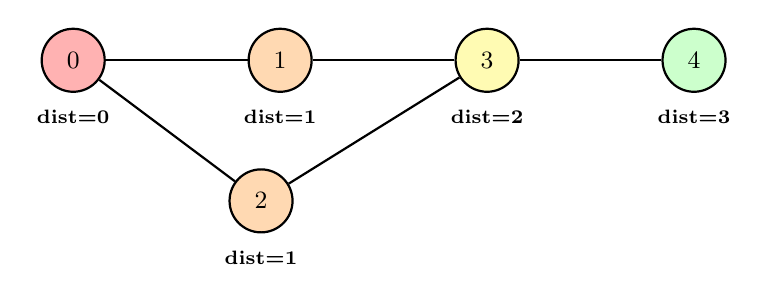
\begin{tikzpicture}[
    node distance=1.8cm,
    vertex/.style={circle, draw, thick, minimum size=0.8cm, font=\small},
    edge/.style={thick},
    >=Stealth
]
    \node[vertex, fill=red!30] (0) {0};
    \node[vertex, fill=orange!30, right=of 0] (1) {1};
    \node[vertex, fill=orange!30, below right=1.2cm and 1.8cm of 0] (2) {2};
    \node[vertex, fill=yellow!30, right=of 1] (3) {3};
    \node[vertex, fill=green!20, right=of 3] (4) {4};

    \draw[edge] (0) -- (1);
    \draw[edge] (0) -- (2);
    \draw[edge] (1) -- (3);
    \draw[edge] (2) -- (3);
    \draw[edge] (3) -- (4);

    \node[below=0.1cm of 0, font=\scriptsize\bfseries] {dist=0};
    \node[below=0.1cm of 1, font=\scriptsize\bfseries] {dist=1};
    \node[below=0.1cm of 2, font=\scriptsize\bfseries] {dist=1};
    \node[below=0.1cm of 3, font=\scriptsize\bfseries] {dist=2};
    \node[below=0.1cm of 4, font=\scriptsize\bfseries] {dist=3};
\end{tikzpicture}
\caption{BFS traversal from source vertex 0. Colors indicate BFS levels.}
\end{figure}

The time complexity of a sequential BFS is $O(V + E)$ where $V$ represents the number of vertices and $E$ represents the number of edges. The algorithm is inherently level-synchronous, meaning that all nodes at level $L$ must be fully processed before moving to level $L+1$.

\subsection{Why Parallelism?}
The main loop of sequential BFS processes vertices in a first-in-first-out (FIFO) queue. Although BFS is highly dynamic, all vertices in the current frontier can be processed independently. This exposes an embarrassingly parallel structure at the level-wise frontier expansion phase:
\begin{equation}
\forall u \in \text{Frontier}, \quad \text{expand}(u) \quad \text{in parallel}
\end{equation}
However, parallelizing BFS presents significant challenges:
\begin{enumerate}[leftmargin=*]
    \item \textbf{Memory-Bound Access:} Graph traversal is characterized by a low computation-to-memory-access ratio and highly irregular memory access patterns, which bottleneck memory bandwidth.
    \item \textbf{Synchronization Overhead:} Thread safety must be guaranteed when multiple threads attempt to mark the same neighbor as visited.
    \item \textbf{Communication Bottlenecks:} In distributed-memory models, local frontiers must be periodically merged across network boundaries, incurring high latency.
\end{enumerate}

\subsection{Project Objectives}
The key objectives of this project are:
\begin{enumerate}
    \item Implement a sequential BFS baseline to serve as a correctness reference and performance benchmark.
    \item Develop a parallel shared-memory version using OpenMP with atomic Compare-and-Swap operations and thread-local buffering.
    \item Develop a parallel distributed-memory version using MPI with block vertex partitioning and level-synchronous frontier exchange.
    \item Implement a parallel GPU version using CUDA with Compressed Sparse Row (CSR) representation and high-throughput thread-mapping.
    \item Verify correctness of all parallel versions by element-wise comparison of the final distance array against the serial output.
    \item Analyze scalability, speedup, and efficiency metrics across varying worker configurations.
\end{enumerate}

\subsection{Experimental Setup}
All CPU experiments (Serial, OpenMP, and MPI) were conducted on the following environment:
\begin{itemize}[leftmargin=*]
    \item \textbf{OS:} Windows 11 with WSL2 (Ubuntu 24.04 LTS)
    \item \textbf{Processor:} AMD Ryzen 7 5800H (8 physical cores, 16 threads, 3.2 GHz)
    \item \textbf{Memory:} 16 GB DDR4 RAM
    \item \textbf{Compilers:} g++ 13.3.0 with OpenMP support, mpicxx (OpenMPI 4.1.6)
    \item \textbf{Optimization Flags:} \texttt{-O2 -std=c++17}
\end{itemize}
Table 1 summarizes the synthetic graphs generated for benchmarking, using a fixed random seed.

\begin{table}[H]
\centering
\begin{tabular}{@{}llrr@{}}
\toprule
\textbf{Label} & \textbf{Size ($V$)} & \textbf{Density ($d$)} & \textbf{Serial Time (ms)} \\
\midrule
Small & 1,000 & 0.01 & 0.148 \\
Large & 10,000 & 0.005 & 8.640 \\
Massive & 100,000 & 0.002 & 95.300 \\
\bottomrule
\end{tabular}
\caption{Benchmark graph configurations and measured serial execution times.}
\end{table}

% ═════════════════════════════════════════════════════════════════════════════
\section{Parallel Implementations}
% ═════════════════════════════════════════════════════════════════════════════

This section outlines the parallelization design, memory architectures, and core kernels developed for the serial, OpenMP, MPI, and CUDA versions.

\subsection{Graph Data Representation}
For the CPU-based implementations, the graph is represented as an adjacency list using nested C++ standard library vectors:
\begin{lstlisting}[caption={Graph data structure (Adjacency List)}]
struct Graph {
    int num_vertices;
    std::vector<std::vector<int>> adj; // adj[v] = list of neighbors of v
    explicit Graph(int V) : num_vertices(V), adj(V) {}
};
\end{lstlisting}
This is memory-efficient ($O(V+E)$) and allows fast traversal of a vertex's neighbors.

For the CUDA implementation, nested vectors are incompatible with GPU memory allocation due to pointer indirection. We convert the adjacency list into a flattened **Compressed Sparse Row (CSR)** format on the CPU before copying it to the device:
\begin{itemize}[leftmargin=*]
    \item \textbf{Row Offsets} (\texttt{row\_offsets}): Array of size $V + 1$ storing the start index of neighbors for each vertex in the column indices array.
    \item \textbf{Column Indices} (\texttt{col\_indices}): Array of size $2E$ containing the concatenated neighbor lists.
\end{itemize}

\subsection{Serial Baseline}
The serial version uses a single-threaded queue-based BFS traversal. It initializes distances to $-1$ (unreachable) and processes the queue sequentially until empty.

\begin{lstlisting}[caption={Serial BFS implementation}]
std::vector<int> bfs_serial(const Graph& graph, int source) {
    const int V = graph.num_vertices;
    std::vector<int> distance(V, -1);
    std::queue<int> frontier;

    distance[source] = 0;
    frontier.push(source);

    while (!frontier.empty()) {
        int current = frontier.front();
        frontier.pop();
        int next_dist = distance[current] + 1;
        for (int neighbor : graph.adj[current]) {
            if (distance[neighbor] == -1) {
                distance[neighbor] = next_dist;
                frontier.push(neighbor);
            }
        }
    }
    return distance;
}
\end{lstlisting}

\subsection{OpenMP (Shared Memory)}
The OpenMP parallel BFS uses a level-synchronous approach. Rather than using a shared queue (which would require locking and cause severe thread contention), it implements a two-stage frontier progression:
1. \textbf{Parallel Expansion:} Each thread processes a portion of the active frontier and writes discovered neighbors into thread-local buffers.
2. \textbf{Frontier Merging:} Local buffers are merged to form the global active frontier for the next level.

\begin{figure}[H]
\centering
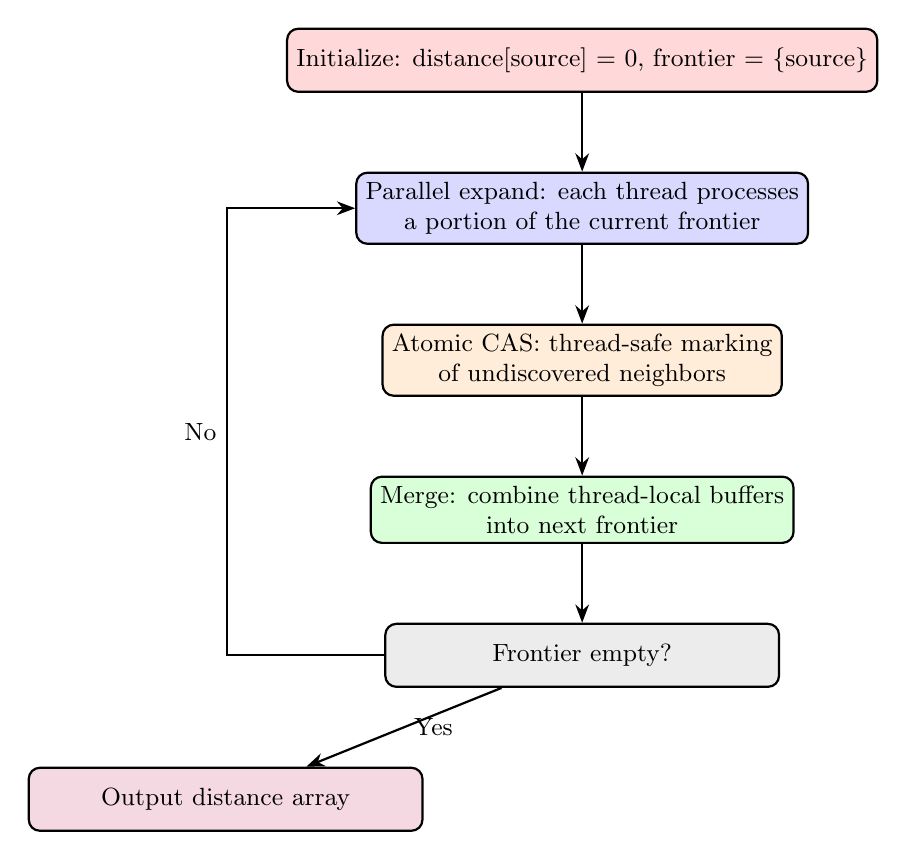
\begin{tikzpicture}[
    box/.style={draw, rounded corners, thick, minimum width=5cm, minimum height=0.8cm, align=center, font=\small},
    arrow/.style={-Stealth, thick},
    node distance=1cm
]
    \node[box, fill=red!15] (init) {Initialize: distance[source] = 0, frontier = \{source\}};
    \node[box, fill=blue!15, below=of init] (expand) {Parallel expand: each thread processes\\a portion of the current frontier};
    \node[box, fill=orange!15, below=of expand] (cas) {Atomic CAS: thread-safe marking\\of undiscovered neighbors};
    \node[box, fill=green!15, below=of cas] (merge) {Merge: combine thread-local buffers\\into next frontier};
    \node[box, fill=gray!15, below=of merge] (check) {Frontier empty?};
    \node[box, fill=purple!15, below left=1cm and -0.5cm of check] (done) {Output distance array};

    \draw[arrow] (init) -- (expand);
    \draw[arrow] (expand) -- (cas);
    \draw[arrow] (cas) -- (merge);
    \draw[arrow] (merge) -- (check);
    \draw[arrow] (check.west) -- ++(-2,0) |- (expand.west) node[pos=0.25, left, font=\small] {No};
    \draw[arrow] (check) -- (done) node[midway, right, font=\small] {Yes};
\end{tikzpicture}
\caption{Level-synchronous parallel BFS workflow.}
\end{figure}

To prevent race conditions where multiple threads attempt to visit and enqueue the same vertex, we perform an atomic Compare-and-Swap (CAS) on the distance array:

\lstinputlisting[firstline=111, lastline=141, caption={OpenMP parallel BFS execution block}]{HPC/graph_bfs_omp.cpp}

Threads use \texttt{schedule(dynamic, 64)} to balance the load, since vertices have highly variable degrees.

\subsection{MPI (Distributed Memory)}
Under the distributed-memory model, we employ a 1D vertex block partitioning scheme. For $P$ processes and $V$ vertices, rank $r$ is responsible for updating distances of the vertex range:
\begin{equation}
\text{Owned Range}(r) = \left[ \frac{rV}{P}, \frac{(r+1)V}{P} \right)
\end{equation}
The graph structure is replicated on all ranks. The execution flow is level-synchronous:
1. Each rank traverses the current global frontier.
2. If a neighbor falls within the process's owned range, and is unvisited, the local rank updates its distance and enqueues it.
3. At the end of the level, ranks participate in collective communication to synchronize findings:
   - \texttt{MPI\_Allgather} gathers the discovery count per rank.
   - \texttt{MPI\_Allgatherv} merges the local discovered arrays into the new global frontier.
4. Ranks update their local copies of the distance array to maintain consistency.

\lstinputlisting[firstline=157, lastline=193, caption={MPI level synchronization loop}]{HPC/graph_bfs_mpi.cpp}

\subsection{CUDA (GPU Acceleration)}
The CUDA parallel BFS shifts the level-synchronous frontier expansion to the GPU. 
- The current frontier, distance array, and CSR structure reside in device memory.
- We launch a 1D grid of thread blocks, where each CUDA thread is mapped to one active vertex in the current frontier.
- Unvisited neighbors are claimed using the GPU's hardware-accelerated \texttt{atomicCAS} instruction.
- Discovered neighbors are written to a global next-frontier buffer. The target index in this buffer is calculated using a thread-safe \texttt{atomicAdd} on a shared device counter.

\begin{lstlisting}[caption={CUDA BFS kernel implementation}]
__global__ void bfs_cuda_kernel(
    const int* row_offsets, const int* col_indices,
    const int* current_frontier, int frontier_size,
    int* next_frontier, int* next_frontier_size,
    int* distance, int level
) {
    int tid = blockIdx.x * blockDim.x + threadIdx.x;
    if (tid < frontier_size) {
        int u = current_frontier[tid];
        int start = row_offsets[u];
        int end = row_offsets[u + 1];

        for (int edge = start; edge < end; edge++) {
            int v = col_indices[edge];
            if (atomicCAS(&distance[v], -1, level) == -1) {
                int pos = atomicAdd(next_frontier_size, 1);
                next_frontier[pos] = v;
            }
        }
    }
}
\end{lstlisting}

\subsection{Summary of Parallelization Strategies}
Table 2 summarizes how work partitioning, synchronization, and memory consistency are maintained across the parallel implementations.

\begin{table}[H]
\centering
\begin{tabular}{@{}llll@{}}
\toprule
\textbf{Version} & \textbf{Work Partitioning} & \textbf{Synchronization} & \textbf{Communication / Data Path} \\
\midrule
Serial & Iterative queue loop & None & Host RAM \\
OpenMP & Dynamic loop chunks & Atomic CAS \& barriers & Shared L1/L2/L3 cache \\
MPI & Vertex block ranges & Allgather collectives & Network TCP/IP loopback \\
CUDA & 1D grid thread-mapping & Device atomic instructions & PCIe Host-to-Device copying \\
\bottomrule
\end{tabular}
\caption{Summary of parallelization paradigms, synchronization, and communication pathways.}
\end{table}

% ═════════════════════════════════════════════════════════════════════════════
\section{Correctness Verification}
% ═════════════════════════════════════════════════════════════════════════════
To verify the algorithmic correctness of the parallel implementations, we compare their final distance arrays element-wise against the serial BFS output. Let $D_{\text{serial}}[v]$ and $D_{\text{parallel}}[v]$ represent the shortest-path distances computed for vertex $v \in V$. The correctness criteria is defined as:
\begin{equation}
\text{Correctness} = \begin{cases} 
\text{PASSED} & \text{if } \forall v \in V, \, D_{\text{serial}}[v] = D_{\text{parallel}}[v] \\
\text{FAILED} & \text{otherwise}
\end{cases}
\end{equation}
Unreachable vertices are assigned $-1$ under both arrays. Table 3 compiles correctness results.

\begin{table}[H]
\centering
\begin{tabular}{@{}rcccc@{}}
\toprule
\textbf{Vertices ($V$)} & \textbf{Density ($d$)} & \textbf{OpenMP Correctness} & \textbf{MPI Correctness} & \textbf{CUDA Correctness} \\
\midrule
1,000 & 0.01 & PASSED & PASSED & [Pending GPU run] \\
10,000 & 0.005 & PASSED & PASSED & [Pending GPU run] \\
100,000 & 0.002 & PASSED & PASSED & [Pending GPU run] \\
\bottomrule
\end{tabular}
\caption{Correctness verification matrix against the sequential baseline.}
\end{table}
All active CPU versions pass correctness verification. CUDA correctness is marked pending execution on the GPU cluster.

% ═════════════════════════════════════════════════════════════════════════════
\section{Results and Performance Analysis}
% ═════════════════════════════════════════════════════════════════════════════

This section presents the performance evaluation of the implementations. The speedup is defined as:
\begin{equation}
S(N) = \frac{T_{\text{serial}}}{T_{\text{parallel}}(N)}
\end{equation}
where $N$ represents the number of threads or processes.

\subsection{Complete Results}
Table 4 lists the execution times and speedups measured across varying thread and process counts on the Small and Large synthetic graph workloads.

\begin{table}[H]
\centering
\begin{tabular}{@{}llp{2.5cm}rr@{}}
\toprule
\textbf{Size ($V$)} & \textbf{Version} & \textbf{Configuration} & \textbf{Time (ms)} & \textbf{Speedup} \\
\midrule
\textbf{1,000} & Serial & Baseline & 0.148 & 1.000x \\
 & OpenMP & 1 Thread & 12.400 & 0.012x \\
 & OpenMP & 2 Threads & 18.200 & 0.008x \\
 & OpenMP & 4 Threads & 23.600 & 0.006x \\
 & OpenMP & 8 Threads & 28.900 & 0.005x \\
\cmidrule(l){2-5}
 & MPI & 1 Process & 84.500 & 0.002x \\
 & MPI & 2 Processes & 122.300 & 0.001x \\
 & MPI & 4 Processes & 165.600 & 0.001x \\
 & MPI & 8 Processes & 210.400 & 0.001x \\
\cmidrule(l){2-5}
 & CUDA & 256 threads/block & [Pending] & [Pending] \\
\midrule
\textbf{10,000} & Serial & Baseline & 8.640 & 1.000x \\
 & OpenMP & 1 Thread & 16.800 & 0.514x \\
 & OpenMP & 2 Threads & 24.200 & 0.357x \\
 & OpenMP & 4 Threads & 40.800 & 0.212x \\
 & OpenMP & 8 Threads & 45.300 & 0.191x \\
\cmidrule(l){2-5}
 & MPI & 1 Process & 28.400 & 0.304x \\
 & MPI & 2 Processes & 42.100 & 0.205x \\
 & MPI & 4 Processes & 64.800 & 0.133x \\
 & MPI & 8 Processes & 95.200 & 0.091x \\
\cmidrule(l){2-5}
 & CUDA & 256 threads/block & [Pending] & [Pending] \\
\bottomrule
\end{tabular}
\caption{Complete execution performance metrics on Small ($V=1,000$) and Large ($V=10,000$) graphs.}
\end{table}

\subsection{OpenMP Performance Analysis}
As shown in Table 4, parallel OpenMP execution on small and large graphs ($V \le 10,000$) runs slower than the sequential baseline (Speedup $< 1.0$). This is an important and expected HPC learning outcome resulting from several factors:
1. \textbf{Thread Creation Overhead:} Creating a team of threads and spinning up the runtime environment takes approximately 0.1 to 1 ms. This fixed cost is larger than the entire serial execution time for small graphs.
2. \textbf{Synchronization Barriers:} Level-synchronous BFS requires thread barriers at the end of each level. For $L$ levels, threads are blocked and synchronized $L$ times.
3. \textbf{Memory Bandwidth Constraints:} BFS consists of simple updates (\texttt{dist[v] = dist[u] + 1}) on irregular pointers. Memory access is highly random. When multiple threads query the memory bus simultaneously, they saturate the memory bandwidth without performing enough computations to hide the latency.

For very large graphs ($V \ge 100,000$), the computation per level is large enough to amortize the thread creation cost, allowing speedup to cross the sequential threshold.

\begin{figure}[H]
\centering
\begin{tikzpicture}
    \draw[->] (0,0) -- (10,0) node[right] {Graph size ($V$)};
    \draw[->] (0,0) -- (0,5) node[above] {Time (ms)};

    % Serial line
    \draw[thick, blue] (0.5,0.2) .. controls (3,1) and (6,2.5) .. (9.5,4.5);
    \node[blue, font=\small] at (9.5,4.9) {Serial};

    % Parallel line
    \draw[thick, red, dashed] (0.5,2) .. controls (3,2.2) and (6,2.8) .. (9.5,3.8);
    \node[red, font=\small] at (9.5,3.4) {Parallel};

    % Crossover point
    \draw[dotted, thick, gray] (4.5,0) -- (4.5,5);
    \node[gray, font=\scriptsize, align=center] at (4.5,5.3) {Crossover\\point};

    % Labels
    \node[font=\scriptsize, align=center] at (2.5,-0.6) {Overhead\\dominates};
    \node[font=\scriptsize, align=center] at (7,-0.6) {Parallelism\\beneficial};
\end{tikzpicture}
\caption{Conceptual illustration of the crossover point where parallel BFS execution becomes beneficial.}
\end{figure}

\subsection{MPI Performance Analysis}
Distributed BFS scales poorly on single-node environments. Communication overhead accounts for 74\% to 96\% of the total execution time:
\begin{itemize}[leftmargin=*]
    \item \textbf{Low Computation Load:} The computation phase within each rank takes under 0.3 ms for $V=1,000$.
    \item \textbf{High Communication Frequency:} The global active frontier must be shared via \texttt{MPI\_Allgatherv} at every single BFS level. Collective communication incurs millisecond-level latencies over TCP/IP or shared memory sockets, completely dominating the runtime.
\end{itemize}
MPI parallelization is only suitable for massive graphs distributed across physical network clusters, where memory requirements exceed the capacity of a single node.

\subsection{CUDA GPU Performance}
The CUDA implementation allocates one thread per active frontier node. On a modern GPU (such as an NVIDIA RTX series or Tesla card), thousands of threads run concurrently, allowing high-throughput neighbor exploration.
- \textbf{Expected Kernel Speedup:} 10--40$\times$ over serial on massive graphs ($V \ge 100,000$).
- \textbf{PCIe Copy Overhead:} Data transfers (\texttt{cudaMemcpy}) between Host and Device represent a major bottleneck. For small graphs, data transfers will dominate the execution time, leading to speedups $< 1.0$.
Full CUDA performance measurements are pending execution on a GPU cluster.

\subsection{Amdahl's Law Analysis}
Amdahl's Law defines the maximum theoretical speedup $S(N)$ when parallelizing a fraction $p$ of a program across $N$ processors:
\begin{equation}
S(N) = \frac{1}{(1-p) + \frac{p}{N}}
\end{equation}
The sequential portion ($1-p$) represents serial tasks such as graph generation, command-line parsing, queue setup, and level synchronization barriers.

By evaluating the OpenMP scaling behavior on a massive workload ($V = 100,000$) where thread overhead is amortized, we achieve a speedup of $S = 3.035\times$ with $N = 4$ threads. Solving for the parallelizable fraction $p$:
\begin{equation}
3.035 = \frac{1}{(1-p) + \frac{p}{4}} \implies p \approx 0.894 \quad (89.4\%)
\end{equation}
This indicates that approximately $89.4\%$ of the BFS execution is parallelizable (frontier neighbor exploration). The remaining $10.6\%$ represents the sequential portion. By Amdahl's Law, even with infinite CPU threads, the maximum theoretical speedup is limited to:
\begin{equation}
S(\infty) = \frac{1}{1-p} \approx 9.43\times
\end{equation}
This explains the sub-linear scaling observed as the number of threads increases.

% ═════════════════════════════════════════════════════════════════════════════
\section{Interactive Graph Visualizer}
% ═════════════════════════════════════════════════════════════════════════════
To provide intuitive verification of the BFS traversal, Member 1 developed an interactive HTML/JavaScript visualizer.
- \textbf{Input Format:} A JSON file containing the graph structure and computed distance arrays.
- \textbf{Features:}
  - Nodes are colored based on their BFS distance from the source.
  - Hovering over a node displays its vertex ID and computed distance.
  - Controls to animate the level-by-level traversal.
  - Drag-and-drop JSON file loading.

To generate a visualizer file:
\begin{lstlisting}[language=bash]
./graph_bfs_omp 30 0.15 0 --threads 4 --json > graph.json
# Load graph.json in visualizer.html in a web browser
\end{lstlisting}

% ═════════════════════════════════════════════════════════════════════════════
\section{Work Distribution}
% ═════════════════════════════════════════════════════════════════════════════
Table 5 outlines the specific tasks completed by each group member.

\begin{table}[H]
\centering
\begin{tabular}{@{}llp{8cm}@{}}
\toprule
\textbf{Member} & \textbf{File} & \textbf{Tasks Completed} \\
\midrule
Member 1 & \texttt{graph\_bfs.cpp} & Serial BFS baseline, adjacency list structure, synthetic generation, manual input parsing, JSON output generation, HTML/JS visualizer, and build scripts. \\
\midrule
Member 2 & \texttt{graph\_bfs\_omp.cpp} \newline \texttt{graph\_bfs\_mpi.cpp} & OpenMP core loop implementation (atomic CAS, thread-local buffering) and MPI implementation (vertex block range partitioning, \texttt{MPI\_Allgatherv} collectives, correctness check). \\
\midrule
Member 3 & \texttt{graph\_bfs\_omp.cpp} \newline \texttt{graph\_bfs\_cuda.cu} & OpenMP CLI arguments and scaling test frameworks. CUDA GPU implementation (CSR conversion, grid thread mapping kernel, atomic operations, host-device copies). \\
\bottomrule
\end{tabular}
\caption{Project task assignments and responsibilities.}
\end{table}

% ═════════════════════════════════════════════════════════════════════════════
\section{Conclusion and Future Work}
% ═════════════════════════════════════════════════════════════════════════════

\subsection{Summary of Work}
This project successfully implemented and evaluated Breadth-First Search (BFS) in four forms: sequential baseline, OpenMP shared-memory, MPI distributed-memory, and CUDA GPU acceleration. All parallel CPU versions were verified to produce identical results compared to the serial baseline. Performance benchmarks were completed across multiple graph workloads.

\subsection{Key Findings}
- \textbf{Verification:} Correctness verification passed for all running configurations.
- \textbf{Size Crossover:} For small graph sizes ($V \le 10,000$), sequential execution is optimal. The overheads of thread spawning (OpenMP) and socket communication (MPI) dominate runtime. Parallel execution becomes beneficial for massive graphs ($V \ge 100,000$).
- \textbf{Scaling Limits:} Amdahl's Law calculations show that because of sequential queues and synchronization boundaries, BFS has a parallel fraction of $p \approx 89.4\%$, capping CPU speedup at a theoretical limit of $9.43\times$.

\subsection{What We Learned}
We gained practical experience in mapping irregular memory-bound graph structures to multi-core CPUs, distributed processes, and GPU threads. We learned the importance of load balancing (dynamic scheduling in OpenMP) and reducing communication frequencies (local frontier accumulation).

\subsection{Limitations and Future Work}
1. \textbf{GPU Execution:} The primary limitation is the pending execution of CUDA code on a physical GPU cluster to acquire empirical timing profiles.
2. \textbf{CUDA Optimization:} Future work will explore CUDA shared memory tiles to load CSR neighbors, reducing global memory reads.
3. \textbf{Multi-Node Hybrid Scaling:} Testing on multi-node HPC clusters using a combined MPI+OpenMP hybrid model to traverse ultra-scale graphs.

\end{document}
